% Compile with XeLaTeX (twice) or Tectonic. UTF-8 source.
\documentclass[11pt,a4paper]{article}
\usepackage[margin=22mm,top=23mm,bottom=23mm,headheight=15pt]{geometry}
\usepackage{fontspec}
\setmainfont{texgyretermes-regular.otf}[BoldFont=texgyretermes-bold.otf,ItalicFont=texgyretermes-italic.otf,BoldItalicFont=texgyretermes-bolditalic.otf]
\setsansfont{texgyreheros-regular.otf}[BoldFont=texgyreheros-bold.otf]
\setmonofont{lmmono10-regular.otf}
\usepackage{amsmath,amssymb,graphicx,booktabs,tabularx,array}
\usepackage[table]{xcolor}
\usepackage{enumitem,fancyhdr,titlesec,caption,float,listings}
\usepackage{tikz}
\usetikzlibrary{arrows.meta,positioning,shapes.geometric}
\usepackage{hyperref}
\usepackage{bookmark}
\definecolor{Navy}{HTML}{16324F}
\definecolor{Teal}{HTML}{087E8B}
\definecolor{Pale}{HTML}{EDF5F7}
\definecolor{Muted}{HTML}{526273}
\definecolor{Rule}{HTML}{CCD9E2}
\hypersetup{colorlinks=true,linkcolor=Navy,citecolor=Teal,urlcolor=Teal,pdftitle={Định hướng số hóa sơ đồ điện từ ảnh và PDF scan},pdfauthor={Báo cáo kỹ thuật},bookmarksnumbered=true}
\urlstyle{same}
\renewcommand{\contentsname}{Mục lục}
\renewcommand{\refname}{Tài liệu tham khảo}
\renewcommand{\figurename}{Hình}
\renewcommand{\tablename}{Bảng}
\renewcommand{\lstlistingname}{Ví dụ}
\setcounter{tocdepth}{1}
\setlength{\parindent}{0pt}
\setlength{\parskip}{5pt}
\linespread{1.08}
\setlength{\emergencystretch}{3em}
\setlist[itemize]{leftmargin=5mm,itemsep=2pt,topsep=3pt}
\setlist[enumerate]{leftmargin=6mm,itemsep=2pt,topsep=3pt}
\newcolumntype{Y}{>{\raggedright\arraybackslash}X}
\renewcommand{\arraystretch}{1.22}
\captionsetup{font=small,labelfont=bf,skip=6pt}
\titleformat{\section}{\Large\sffamily\bfseries\color{Navy}}{\thesection}{0.6em}{}
\titleformat{\subsection}{\large\bfseries\color{Navy}}{\thesubsection}{0.6em}{}
\titlespacing*{\section}{0pt}{9pt}{8pt}
\titlespacing*{\subsection}{0pt}{7pt}{3pt}
\pagestyle{fancy}
\fancyhf{}
\fancyhead[L]{\small\sffamily\color{Muted}SỐ HÓA SƠ ĐỒ ĐIỆN TỪ ẢNH}
\fancyhead[R]{\small\sffamily\color{Muted}Định hướng kỹ thuật}
\fancyfoot[L]{\small\color{Muted}Phiên bản 1.0 | 24/09/2026}
\fancyfoot[R]{\small\thepage}
\renewcommand{\headrulewidth}{0.4pt}
\newcommand{\decision}[1]{\par\smallskip\noindent\colorbox{Pale}{\parbox{\dimexpr\linewidth-2\fboxsep\relax}{\textbf{Đề xuất:} #1}}\par\smallskip}
\newcommand{\code}[1]{\texttt{\detokenize{#1}}}
\lstset{basicstyle=\ttfamily\footnotesize,breaklines=true,columns=fullflexible,keepspaces=true,showstringspaces=false,frame=single,rulecolor=\color{Rule},backgroundcolor=\color{Pale},xleftmargin=2mm,xrightmargin=2mm,aboveskip=5pt,belowskip=5pt}

\begin{document}
\hypersetup{pageanchor=false}
\begin{titlepage}
\color{Navy}
\vspace*{10mm}
{\sffamily\large BÁO CÁO ĐỊNH HƯỚNG KỸ THUẬT\par}
\vspace{8mm}
{\sffamily\bfseries\fontsize{29}{36}\selectfont Số hóa sơ đồ điện\\từ ảnh và PDF scan\par}
\vspace{6mm}
{\Large Ứng dụng Computer Vision để trích xuất thiết bị,\\nét vẽ SVG và quan hệ đấu nối\par}
\vspace{10mm}
{\color{Teal}\rule{\linewidth}{1.3pt}}
\vspace{7mm}
\begin{tikzpicture}[node distance=7mm,box/.style={draw=Rule,fill=Pale,rounded corners=2mm,text width=42mm,minimum height=19mm,align=center,font=\sffamily\small},arr/.style={-{Stealth[length=2mm]},thick,Teal}]
\node[box] (a) {Ảnh đầu vào\\và thư viện ký hiệu};
\node[box,right=of a] (b) {Nhận dạng thiết bị\\và đường dây};
\node[box,right=of b] (c) {JSON + SVG\\và đồ thị đấu nối};
\draw[arr] (a)--(b); \draw[arr] (b)--(c);
\end{tikzpicture}
\vfill
\color{black}
\begin{tabularx}{\linewidth}{@{}p{34mm}Y@{}}
\textbf{Bối cảnh} & Công ty nhỏ; đầu vào không có cấu trúc CAD; ưu tiên khả năng triển khai, kiểm tra và mở rộng.\\
\textbf{Phạm vi} & Xác định bài toán, phân rã nhiệm vụ, lựa chọn thuật toán, tích hợp hệ thống và kế hoạch đánh giá.\\
\textbf{Trạng thái} & Đề xuất thiết kế; chưa huấn luyện mô hình hoặc đo độ chính xác trên bộ dữ liệu công ty.\\
\textbf{Ngày lập} & 24 tháng 09 năm 2026.\\
\end{tabularx}\par
\vspace{6mm}
{\small\raggedright\color{Muted}Ảnh minh họa do người dùng cung cấp. Tọa độ và JSON trong báo cáo là ví dụ thiết kế.\par}
\end{titlepage}

\pagenumbering{roman}
\hypersetup{pageanchor=true}
\section*{Tóm tắt định hướng}
\addcontentsline{toc}{section}{Tóm tắt định hướng}
Bài toán cần giải là chuyển sơ đồ điện ở dạng ảnh thành tập đối tượng có thể chỉnh sửa và dữ liệu có thể xử lý bằng máy. Mỗi thiết bị cần có vị trí, loại, nhãn và hình vẽ; mỗi dây cần có đường đi và đầu nối. Để phục vụ truy vết mạng điện, dữ liệu hình học phải được bổ sung bằng quan hệ đấu nối.

Giải pháp đề xuất là một quy trình kết hợp: CV cổ điển xử lý ảnh và đường dây; so khớp mẫu tạo kết quả đối chứng ban đầu; detector nhỏ nhận dạng ký hiệu khi có đủ dữ liệu; OCR đọc nhãn; các quy tắc hình học và nghiệp vụ dựng đồ thị. VLM chỉ được thử nghiệm cho những trường hợp chưa rõ. Giao diện kiểm tra, sửa lỗi là một phần của sản phẩm.

\decision{Triển khai trước trên một họ sơ đồ và bộ ký hiệu được xác nhận. Chỉ bổ sung mô hình phức tạp khi kết quả đánh giá chứng minh giảm được lỗi hoặc thời gian sửa. Không dùng độ giống hình SVG làm đại diện cho độ đúng của đấu nối.}

\begingroup
\small
\setlength{\parskip}{0pt}
\linespread{1}\selectfont
\tableofcontents
\endgroup
\clearpage
\pagenumbering{arabic}

\section{Xác định bài toán và phạm vi}
\subsection{Mục tiêu}
Cho ảnh sơ đồ điện và tài liệu ký hiệu tham chiếu, hệ thống cần phân tích thành các đối tượng riêng biệt, phục hồi bố cục và xây dựng các liên kết có bằng chứng. Đây là bài toán kết hợp \textit{phân tích tài liệu kỹ thuật}, \textit{nhận dạng đối tượng} và \textit{khôi phục cấu trúc đồ thị}.

Có thể biểu diễn ánh xạ mục tiêu như sau:
\begin{equation}
F(I,\mathcal{L},\mathcal{R})=(\mathcal{O},\mathcal{W},\mathcal{T},\mathcal{G},\mathcal{U}),
\end{equation}
trong đó $I$ là ảnh; $\mathcal{L}$ là thư viện ký hiệu; $\mathcal{R}$ là quy ước bản vẽ; $\mathcal{O}$ là thiết bị; $\mathcal{W}$ là dây; $\mathcal{T}$ là văn bản; $\mathcal{G}$ là cấu trúc đấu nối; $\mathcal{U}$ là tập trường hợp chưa xác định.

\begin{figure}[H]
\centering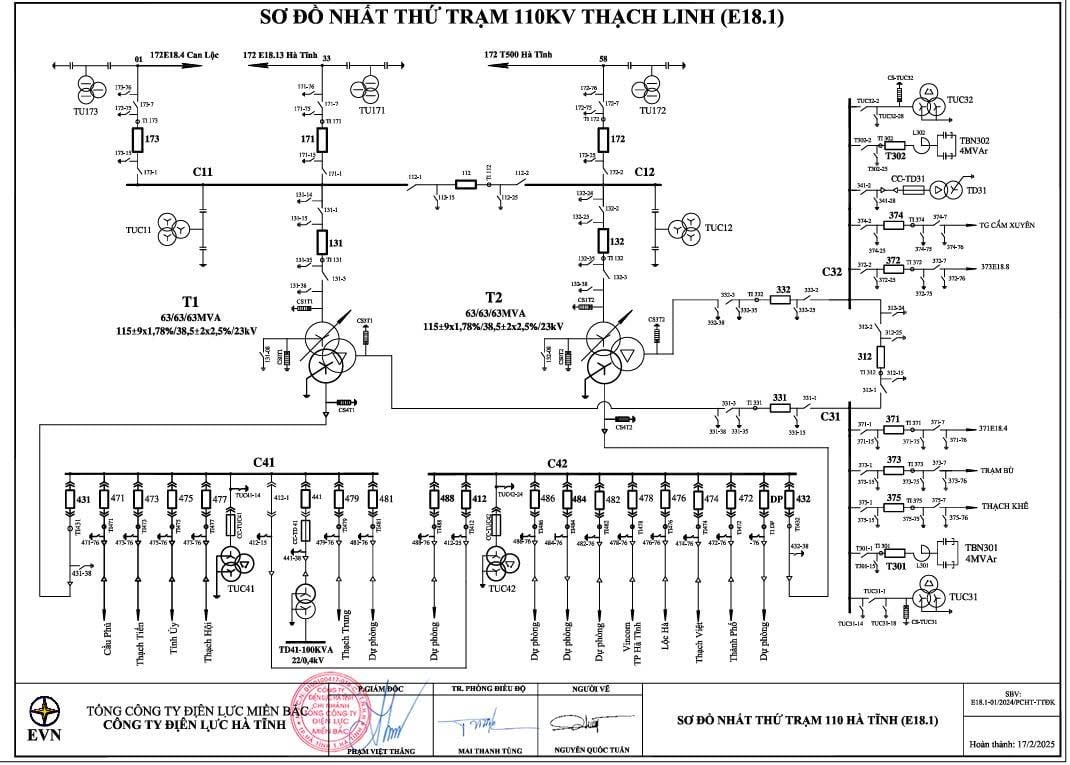
\includegraphics[width=0.94\linewidth]{assets/so_do_nguon.png}
\caption{Sơ đồ minh họa do người dùng cung cấp. Ảnh được dùng để phân tích đặc điểm bài toán, chưa được nhận dạng tự động trong báo cáo này.}
\end{figure}

\subsection{Ba mức kết quả cần phân biệt}
\begin{enumerate}
\item \textbf{Hình học:} các nét, chữ và vị trí được biểu diễn lại bằng SVG.
\item \textbf{Ngữ nghĩa:} các nét được gom thành thiết bị có loại, nhãn và đầu cực.
\item \textbf{Đấu nối:} hệ thống biết dây nào nối tới đầu cực nào, giao điểm nào thực sự nối điện.
\end{enumerate}
Chuyển ảnh thành vector chỉ đáp ứng một phần mức thứ nhất. Phạm vi ban đầu không bao gồm tính toán trào lưu công suất, xác nhận trạng thái vận hành thời gian thực hoặc tự lập phương án thao tác điện. Các chức năng đó cần dữ liệu và kiểm chứng bổ sung.

\clearpage
\section{Đặc tả đầu vào và đầu ra}
\subsection{Đầu vào}
\begin{tabularx}{\linewidth}{@{}p{33mm}Y@{}}
\toprule
\textbf{Thành phần} & \textbf{Nội dung và yêu cầu}\\\midrule
Ảnh/PDF scan & PNG, JPEG, TIFF hoặc trang PDF chứa ảnh. Lưu tệp gốc, mã tài liệu, số trang, kích thước pixel và độ phân giải nếu biết.\\
Thư viện ký hiệu & Mẫu ảnh hoặc SVG, tên loại, các biến thể, hướng, số đầu cực và vị trí đầu cực theo hệ tọa độ mẫu.\\
Quy ước bản vẽ & Cách biểu diễn giao chéo, điểm nối, tiếp địa, trạng thái đóng/cắt và quy tắc đặt mã. Phạm vi áp dụng phải gắn với từng họ sơ đồ.\\
Dữ liệu học/đánh giá & Bounding box, loại thiết bị, nhãn chữ, đầu cực, dây và quan hệ nối do người có chuyên môn xác nhận. Cần nếu huấn luyện hoặc đo chất lượng.\\\bottomrule
\end{tabularx}

Bảng ký hiệu điện cơ bản được cung cấp chưa bao phủ đầy đủ ký hiệu sơ đồ nhất thứ trạm điện. Cần thống nhất danh mục trước khi gán nhãn. Ảnh mờ phải được đánh dấu chất lượng thấp; phóng lớn hoặc tăng DPI khi raster hóa PDF không phục hồi thông tin đã mất trong ảnh scan.

\subsection{Đầu ra}
\begin{tabularx}{\linewidth}{@{}p{30mm}Y@{}}
\toprule
\textbf{Đối tượng} & \textbf{Các thuộc tính cần lưu}\\\midrule
Thiết bị & ID ổn định; loại; nhãn; vùng bao; vị trí, tỷ lệ và góc xoay; SVG hoặc tham chiếu mẫu; danh sách đầu cực.\\
Đường dây & ID; chuỗi điểm hình học; điểm đầu/cuối; tham chiếu đầu cực hoặc nút nối; bằng chứng trên ảnh gốc.\\
Văn bản & Nội dung OCR thô, nội dung đã xác nhận, vùng bao, hướng, liên kết tới thiết bị nếu có.\\
Nút/quan hệ & Nút nối, nhánh rẽ, giao chéo không nối, thanh cái, kết nối đầu cực. Không hợp nhất nút chỉ vì cùng tọa độ.\\
Thông tin kiểm tra & Nguồn và phiên bản xử lý; độ tin cậy theo từng nhiệm vụ; trạng thái kiểm tra; lý do cần sửa; lịch sử chỉnh sửa.\\\bottomrule
\end{tabularx}

\subsection{Hệ tọa độ và định dạng trao đổi}
Chọn hệ tọa độ trang chuẩn: gốc trên trái, $x$ tăng sang phải, $y$ tăng xuống dưới, đơn vị pixel. Mọi phép cắt ô, xoay và thu phóng phải lưu biến đổi về trang nguồn. Ký hiệu mẫu dùng tọa độ cục bộ; đầu cực được biến đổi cùng ký hiệu.

\textbf{JSON} là dữ liệu cấu trúc chính; \textbf{SVG} là biểu diễn để hiển thị và tương tác. Mỗi nhóm SVG có ID khớp với JSON. Tách \textit{trạng thái được vẽ}, \textit{trạng thái vận hành} và \textit{trạng thái giả lập}; mặc định là chưa biết nếu không có nguồn xác nhận.

\clearpage
\section{Phân tích và chia nhỏ vấn đề}
\subsection{Các khó khăn đặc thù}
Ký hiệu và nhãn có kích thước nhỏ; nhiều hình tương tự nhau; chữ có thể xoay và dính dây. Dây nối vào thiết bị làm việc tách vùng liên thông trở nên khó khăn. Một chấm hoặc khoảng hở nhỏ có thể thay đổi ý nghĩa đấu nối. Ngoài ra, cùng một loại thiết bị có thể có nhiều cách vẽ giữa các nguồn.

\begin{table}[H]
\centering\small
\begin{tabularx}{\linewidth}{@{}p{8mm}p{34mm}Y Y@{}}
\toprule
\textbf{Mã} & \textbf{Vấn đề con} & \textbf{Kết quả trung gian} & \textbf{Hướng ưu tiên}\\\midrule
P1 & Chất lượng và bố cục & Ảnh chuẩn, vùng sơ đồ, phép biến đổi & CV cổ điển, tách vùng\\
P2 & Phát hiện thiết bị & Vùng bao, loại, hướng & So khớp; detector khi cần\\
P3 & Đọc và gán nhãn & Vùng chữ, nội dung, chủ thể & OCR + ràng buộc hình học\\
P4 & Khôi phục nét dây & Đường tâm, đầu mút, nhánh & Morphology + thinning + dò nét\\
P5 & Suy luận đấu nối & Cực, nút, kết nối, nghi ngờ & Hình học + quy ước điện\\
P6 & Tái tạo đối tượng & JSON và SVG đồng bộ & Mẫu ký hiệu + polyline\\
P7 & Kiểm tra và cải tiến & Kết quả xác nhận, dữ liệu sửa & Giao diện sửa + đánh giá\\\bottomrule
\end{tabularx}
\caption{Phân rã theo đầu ra có thể kiểm tra độc lập.}
\end{table}

\subsection{Vì sao cần kết hợp nhiều phương pháp?}
CV cổ điển phù hợp để đo và truy vết hình học; detector phù hợp để tìm đối tượng có nhiều biến thể; OCR chuyên cho chữ. Quy tắc đồ thị sử dụng các kết quả này để kiểm tra sự nhất quán. Không phương pháp nào trong số đó tự giải quyết đầy đủ cả hình học, ngữ nghĩa và đấu nối.

Nghiên cứu SINA cũng sử dụng kết hợp nhận dạng thiết bị, xử lý liên thông, OCR và VLM trong bài toán ảnh sơ đồ thành netlist \cite{sina}. Đây là tài liệu tham khảo về kiến trúc; miền dữ liệu IC/PCB khác sơ đồ trạm điện, nên không chuyển trực tiếp độ chính xác công bố sang dự án này.

\subsection{Nguyên tắc xử lý sự không chắc chắn}
\begin{itemize}
\item Giữ trạng thái \code{unknown} thay vì ép đối tượng vào một loại không có bằng chứng.
\item Lưu độ tin cậy riêng cho loại, nhãn, hình học và kết nối. Điểm do các mô hình khác nhau sinh ra không mặc nhiên so sánh được.
\item Không tự sửa một kết nối chỉ để làm đồ thị có vẻ hợp lý. Quy tắc nghiệp vụ tạo cảnh báo hoặc ứng viên cần xác nhận.
\item Cho phép một bước sau yêu cầu xem lại vùng ảnh, nhưng giữ phiên bản và giới hạn số lần chạy lại để tránh vòng xử lý không kết thúc.
\end{itemize}

\clearpage
\section{P1: Tiền xử lý ảnh và chuẩn hóa}
\subsection{Quy trình đề xuất}
\begin{enumerate}
\item \textbf{Nạp và kiểm tra nguồn:} lưu bản gốc, kích thước, trang; đo sơ bộ độ mờ, tương phản và độ nghiêng. Ưu tiên lấy ảnh scan nhúng ở độ phân giải gốc nếu khả thi.
\item \textbf{Xác định vùng sơ đồ:} tách khung tên và chữ ký khỏi vùng xử lý. Không xóa đường chỉ vì nó dài hoặc sát biên; đường đó có thể là thanh cái hoặc dây đi vòng.
\item \textbf{Chỉnh hình học:} deskew bằng hướng các đoạn thẳng đáng tin cậy; sửa phối cảnh khi ảnh được chụp nghiêng. Lưu ma trận biến đổi.
\item \textbf{Tạo nhánh ảnh:} ảnh xám ít biến đổi cho OCR/detector; ảnh nhị phân cho dò nét; ảnh gốc để đối chiếu.
\item \textbf{Chia ô chồng lấn:} phục vụ ký hiệu nhỏ; đồng thời giữ ảnh toàn trang để phân tích bố cục, thanh cái và tuyến dây dài.
\end{enumerate}

\subsection{Thuật toán và giới hạn}
\begin{tabularx}{\linewidth}{@{}>{\raggedright\arraybackslash}p{36mm}Y Y@{}}
\toprule
\textbf{Thuật toán} & \textbf{Tác dụng} & \textbf{Giới hạn cần kiểm tra}\\\midrule
Otsu / ngưỡng thích nghi & Tách mực khỏi nền; ngưỡng cục bộ hữu ích với nền không đều & Có thể mất nét mảnh hoặc sinh nhiễu; chọn bằng mẫu scan thực tế\\
Lọc nhiễu nhẹ & Giảm hạt scan trước khi nhị phân hóa & Lọc mạnh làm mất dấu chấm và chi tiết ký hiệu\\
Erosion, dilation, opening, closing & Tách hoặc nối cấu trúc theo phần tử cấu trúc \cite{morph} & Có thể làm thay đổi topology; không closing toàn trang một cách mặc định\\
Hough line & Ước lượng hướng trang, tìm ứng viên đoạn thẳng \cite{hough} & Cạnh ký hiệu và khung bản vẽ cũng tạo đoạn thẳng\\\bottomrule
\end{tabularx}

\subsection{Tiêu chí đánh giá}
Kiểm tra nét mảnh, chấm nối và khe hở trước/sau xử lý. Đánh giá tác động lên nhận dạng và đấu nối thay vì chỉ chấm mức sạch của ảnh. Tham số hình thái nên tham chiếu độ dày nét ước lượng, không cố định một kích thước kernel cho mọi bản scan.

\decision{Dùng CV cổ điển với cường độ biến đổi thấp và lưu các ảnh trung gian. Nếu vùng ảnh không đủ chi tiết để phân biệt ký hiệu, đưa vào kiểm tra thay vì dùng ảnh tăng cường làm bằng chứng duy nhất.}

\clearpage
\section{P2: Nhận dạng thiết bị và đầu cực}
\subsection{So khớp mẫu làm kết quả đối chứng}
Template matching dò một mẫu trong ảnh lớn \cite{template}. Thử mẫu ảnh xám và mẫu cạnh, nhiều tỷ lệ, các hướng xuất hiện thực tế; lọc các dự đoán trùng. Ưu điểm là ít dữ liệu và dễ kiểm tra; hạn chế là nhạy với kiểu nét, chữ/dây chạm ký hiệu và sự thay đổi hình dạng. Mẫu phải lấy từ tập phát triển, không lấy từ tập kiểm tra cuối cùng.

Khi cần so khớp nét, có thể thử khoảng cách Chamfer một chiều:
\begin{equation}
d(T,I)=\frac{1}{|E_T|}\sum_{p\in E_T}D_I(p),
\end{equation}
với $E_T$ là tập điểm cạnh của mẫu sau biến đổi và $D_I$ là bản đồ khoảng cách tới cạnh gần nhất của vùng ảnh. Điểm thấp gợi ý khớp; đây chỉ là điểm hình học, không phải xác suất đúng. Cần thêm giới hạn vùng, tỷ lệ và kiểm tra ngữ cảnh để giảm khớp giả.

\subsection{Detector khi cần bao phủ nhiều biến thể}
Fine-tune một detector nhỏ để dự đoán vùng bao và loại thiết bị. YOLOX là một ứng viên có triển khai và trọng số tham khảo \cite{yolox}; việc chọn mô hình cuối cùng cần dựa trên thử nghiệm và điều kiện tích hợp. Trọng số pretrained trên ảnh thông thường không thay thế dữ liệu ký hiệu của dự án.

Ký hiệu nhỏ cần được xử lý bằng các ô chồng lấn. Công trình SAHI cung cấp cơ sở tham khảo cho suy luận và fine-tuning theo ảnh cắt \cite{sahi}. Phải ánh xạ kết quả về trang và hợp nhất dự đoán trùng; không ghép nhầm hai thiết bị thật nằm sát nhau. Với cấu trúc lớn, bổ sung xử lý toàn trang hoặc nhiều tỷ lệ.

\subsection{Classification, segmentation và đầu cực}
Classifier nhận vùng ảnh đã cắt và trả về loại, không tự tìm vị trí. Vì detector đã dự đoán lớp, chỉ thêm classifier nếu một nhóm nhầm lẫn cụ thể được cải thiện trên tập kiểm tra. Có thể dự đoán hướng hoặc trạng thái ký hiệu bằng nhánh riêng khi đủ dữ liệu.

Bounding box không cho vị trí đầu cực chính xác. Giai đoạn đầu dùng đầu cực từ mẫu và tinh chỉnh bằng nét cục bộ. Với mẫu có điểm $p$, vị trí trên trang là:
\begin{equation}
p_{\mathrm{page}}=A p+t,
\end{equation}
trong đó $A$ chứa quay và tỷ lệ, $t$ là tịnh tiến. Khi lỗi đầu cực trở thành nút thắt, thử mô hình keypoint hoặc segmentation; không cần gán mask toàn bộ thiết bị ngay từ đầu.

\decision{So khớp là baseline; detector là bước mở rộng. Giữ đường đi \code{unknown} cho ký hiệu ngoài danh mục. Đánh giá riêng sai loại, bỏ sót, trùng đối tượng và sai đầu cực.}

\clearpage
\section{P3: OCR, gán nhãn và vai trò VLM}
\subsection{Đọc văn bản bằng OCR}
OCR cần trả lại nội dung và vị trí, không chỉ chuỗi chữ toàn trang. Thử hệ có sẵn như PaddleOCR, gồm các bước tìm vùng chữ và nhận dạng \cite{ppocr,paddle}. Chọn mô hình hỗ trợ tập ký tự thực tế; đánh giá riêng mã thiết bị và tên tiếng Việt.

Giữ vùng chữ ở độ phân giải đủ cao, xử lý hướng đọc theo từng vùng và lưu cả nội dung thô lẫn nội dung xác nhận. Từ điển mã giúp phát hiện trường hợp nghi ngờ, nhưng không được tự tạo mã mới hoặc thay mã hợp lệ chỉ vì gần với mã thường gặp.

\subsection{Gán văn bản cho thiết bị}
Nhãn gần nhất chưa chắc thuộc thiết bị gần nhất. Đề xuất chấm ứng viên dựa trên khoảng cách chuẩn hóa, hướng tương đối, vùng/ngăn lộ và mức phù hợp cấu trúc mã:
\begin{equation}
C_{ij}=\alpha d_{ij}+\beta o_{ij}+\gamma b_{ij}+\delta r_{ij}.
\end{equation}
$C_{ij}$ là chi phí gán nhãn $i$ cho thiết bị $j$; $d$ là khoảng cách, $o$ là lệch hướng, $b$ là khác nhánh/vùng, $r$ là mức không phù hợp quy tắc. Chuẩn hóa các thành phần trước khi chọn trọng số. Dùng ràng buộc một-một khi đúng với vai trò nhãn; tên chung hoặc thông số nhóm cần mô hình quan hệ riêng.

Cho phép không gán nhãn nếu ứng viên yếu hoặc hai lựa chọn gần ngang nhau. Có thể dùng ghép cặp tối ưu với nút giả cho trường hợp không gán; các trường hợp đơn giản dùng luật hình học dễ kiểm tra.

\subsection{VLM là nhánh hỗ trợ tùy chọn}
VLM có thể xét vùng ảnh kèm ngữ cảnh và chọn từ tập ký hiệu/nhãn đã được đánh số. Nó hữu ích để đề xuất cách hiểu khi có ít mẫu hoặc khi cần kết hợp hình và chữ. SINA là một ví dụ tham khảo sử dụng VLM hỗ trợ gán mã trong một pipeline nhiều thành phần \cite{sina}.

Hạn chế là khả năng suy đoán sai, chi phí suy luận và độ lặp lại phụ thuộc mô hình/cấu hình. Không sử dụng lời tự đánh giá độ tin cậy của VLM như xác suất đã hiệu chuẩn. Không giao toàn bộ việc phát hiện tọa độ và quyết định kết nối cho VLM trong phiên bản đầu.

\begin{itemize}
\item Chỉ gửi vùng khó cùng ngữ cảnh cần thiết; cung cấp các lựa chọn hữu hạn.
\item Yêu cầu đầu ra theo schema, có lựa chọn chưa xác định; kiểm tra tính hợp lệ của ID.
\item Lưu mô hình, phiên bản yêu cầu và kết quả; bộ nhớ đệm tránh gọi lại cùng nội dung.
\item Chỉ giữ bước VLM nếu giảm thời gian sửa hoặc tăng độ đúng so với nhánh không dùng VLM.
\end{itemize}

\clearpage
\section{P4: Tách đường dây và khôi phục hình học}
\subsection{Đường tâm là biểu diễn ưu tiên}
Dây raster thường có bề dày, còn dữ liệu hình học cần một đường đi. Skeletonization thu cấu trúc nhị phân về nét mảnh để hỗ trợ truy vết \cite{skeleton}. Nó bảo toàn liên thông của ảnh theo thuật toán, không bảo đảm liên thông đó đúng về điện. Việc vector hóa đường viền có thể tạo hai cạnh song song cho một dây; do đó đường tâm phù hợp hơn với mục tiêu đấu nối.

\subsection{Quy trình xử lý đề xuất}
\begin{enumerate}
\item Tạo mask ứng viên dây từ ảnh nhị phân, nét ngang/dọc và các đoạn khác hướng. Giữ cả dây đi vòng và đoạn xiên.
\item Dùng vùng thiết bị/văn bản để giảm lẫn nét. Không xóa nguyên bounding box nếu trong đó có đầu dây; bảo toàn vùng quanh đầu cực và kiểm tra ảnh gốc.
\item Làm mảnh mask, tìm đầu mút và ứng viên nhánh rẽ. Gom các pixel nhánh gần nhau thành một sự kiện hình học thay vì tạo nhiều nút giả.
\item Truy vết giữa các điểm đặc biệt, rút gọn thành polyline; Hough có thể hỗ trợ làm thẳng các đoạn đáng tin cậy.
\item Ghép đoạn chỉ khi có bằng chứng về hướng, khoảng cách và khoảng trống. Không nối xuyên vùng thiết bị hoặc khe hở có ý nghĩa.
\item Đưa các giao điểm sang bước P5 để phân loại nối/không nối/chưa rõ.
\end{enumerate}

\subsection{Các lỗi cần xử lý có chủ đích}
\begin{tabularx}{\linewidth}{@{}p{41mm}Y@{}}
\toprule
\textbf{Tình huống} & \textbf{Cách xử lý}\\\midrule
Dây đứt do scan & Đề xuất nối cục bộ khi hai đoạn cùng hướng và không có ký hiệu ngắt; lưu quyết định để kiểm tra.\\
Dây gần cạnh thiết bị & Xét mask thiết bị, vị trí cực và nét gốc; không coi mọi cạnh thẳng là dây.\\
Chấm nối nhỏ & Dùng vùng ảnh chưa bị xóa nhiễu mạnh; đối chiếu cả hình dạng và quy ước tài liệu.\\
Chữ dính dây & Tách theo mask và hướng; nếu mất bằng chứng thì giữ đoạn chưa xác định.\\
Thanh cái dài, nhiều nhánh & Giữ đối tượng thanh cái và các điểm đấu nhánh; không gộp tất cả thành một thiết bị không có cấu trúc.\\\bottomrule
\end{tabularx}

\decision{Đánh giá độ đúng đầu mút và đường đi cùng với lỗi kết nối, thay vì chỉ đo độ trùng pixel. Chỉ nâng cấp sang segmentation dây nếu baseline hình học thất bại có hệ thống trên nhiều trang.}

\clearpage
\section{P5: Khôi phục quan hệ đấu nối}
\subsection{Phân biệt đồ thị hình học và mô hình điện}
Đồ thị hình học mô tả nét, đầu mút và giao điểm. Mô hình điện mô tả đầu cực, nút dẫn điện và quan hệ bên trong từng loại thiết bị. Hai dây trùng tọa độ giao nhau chưa chắc thuộc cùng nút điện.

Đề xuất mô hình gồm: thiết bị $D$, đầu cực $P$, nút dẫn $N$ và quan hệ đầu cực thuộc nút. Các dây/thanh cái tạo liên hệ giữa các đầu cực. Quan hệ đi qua máy cắt phụ thuộc trạng thái; quan hệ qua máy biến áp phải có kiểu riêng, không hợp nhất các phía thành một nút dẫn điện.

\begin{figure}[H]
\centering
\begin{tikzpicture}[line width=0.9pt,font=\small]
\draw (0,0)--(3,0); \draw (1.5,-0.7)--(1.5,0.7);
\fill[Teal] (1.5,0) circle (0.09);
\node[align=center] at (1.5,-1.15) {Giao có điểm nối\\ứng viên cùng nút};
\draw (5,0)--(8,0); \draw (6.5,-0.7)--(6.5,-0.20);
\draw (6.5,0.20)--(6.5,0.7);
\draw (6.5,-0.20) .. controls (6.95,-0.15) and (6.95,0.15) .. (6.5,0.20);
\node[align=center] at (6.5,-1.15) {Cầu vượt minh họa\\ứng viên không nối};
\end{tikzpicture}
\caption{Ví dụ hình học minh họa; quyết định phải dựa trên quy ước được xác nhận của từng bản vẽ.}
\end{figure}

\subsection{Các bước dựng kết nối}
\begin{enumerate}
\item Biến đổi đầu cực mẫu về trang, tinh chỉnh trên nét gần thiết bị.
\item Tìm ứng viên đầu dây cho mỗi cực theo khoảng cách và hướng. Ngưỡng thích nghi theo độ dày nét/kích thước ký hiệu.
\item Phân loại giao điểm: nối, giao chéo không nối, hoặc chưa xác định. Chấm nối, cầu vượt, khe hở và cấu trúc nhánh là bằng chứng.
\item Ghép dây, nút và cực theo ràng buộc; giữ các cạnh ứng viên chưa xác nhận riêng với cạnh đã được chấp nhận.
\item Kiểm tra số đầu cực theo loại, nhãn trùng, đoạn treo và kết nối bất thường; đưa ra cảnh báo có vùng ảnh nguồn.
\end{enumerate}

\subsection{Giới hạn của suy luận}
Đầu dây treo có thể là đầu đi sang trang khác hoặc ký hiệu xuất tuyến hợp lệ. Điểm giao thiếu chấm không được tự xem là không nối nếu quy ước chưa rõ. Không lấy sự hoàn chỉnh của đồ thị làm lý do để bịa kết nối. Với liên kết giữa các trang, cần mã tham chiếu rõ hoặc xác nhận thủ công.

\decision{Ưu tiên giảm nối sai và đưa trường hợp mơ hồ vào hàng đợi kiểm tra. Chức năng truy vết có điện sau này chỉ dùng mô hình đã kiểm tra và trạng thái thiết bị có nguồn xác nhận.}

\clearpage
\section{P6--P7: SVG và kiểm tra có con người}
\subsection{Hai cách biểu diễn hình vẽ}
\begin{tabularx}{\linewidth}{@{}p{35mm}Y Y@{}}
\toprule
\textbf{Cách biểu diễn} & \textbf{Ưu điểm} & \textbf{Hạn chế}\\\midrule
Giữ nét trích xuất & Bám sát scan, thuận lợi đối chiếu & Nhiều nét vụn, khó chỉnh sửa đồng nhất; nhiễu cũng bị giữ lại\\
Dựng bằng mẫu SVG & Đối tượng sạch, ít điểm, dễ xoay và đổi trạng thái & Cần nhận đúng loại/hướng; hình chuẩn hóa có thể khác nét gốc\\\bottomrule
\end{tabularx}

Đề xuất dùng mẫu SVG cho thiết bị đã xác định, polyline cho dây và đối tượng text cho nhãn. Giữ bản gốc cùng lớp chồng kết quả để đối chiếu. Ký hiệu chưa nhận dạng được vẫn được lưu dưới dạng vùng nguồn hoặc nét chưa phân loại; không âm thầm thay bằng mẫu gần giống.

\subsection{Đồng bộ dữ liệu}
JSON là nguồn dữ liệu chính, chứa cả hình học và liên kết. SVG được tạo từ JSON bằng bộ dựng xác định. Mỗi thiết bị là một nhóm có ID, phép biến đổi và tham chiếu mẫu. Vị trí hình vẽ và vị trí đầu cực cùng sử dụng một phép biến đổi để tránh sai lệch.

Khi người dùng kéo thiết bị, phần mềm cần cập nhật dây liên quan hoặc đánh dấu kết nối cần kiểm tra. Khi sửa một dây, phải tính lại các quan hệ chịu ảnh hưởng. Sửa hình trên màn hình mà không cập nhật đồ thị sẽ tạo hai phiên bản sự thật.

\subsection{Giao diện tối thiểu}
\begin{itemize}
\item Bật/tắt ảnh gốc, thiết bị, nhãn, dây và điểm nối; phóng to vùng nghi ngờ.
\item Đổi loại/nhãn thiết bị, điều chỉnh vị trí/hướng/cực; nối hoặc tách dây.
\item Danh sách lỗi có lý do: nhãn mơ hồ, đầu cực lệch, ký hiệu lạ, giao điểm chưa rõ.
\item Chấp nhận hoặc từ chối đề xuất; hoàn tác và lưu lịch sử.
\item Đánh dấu xác nhận riêng cho hình học, nhãn và đấu nối.
\end{itemize}

\subsection{Phản hồi thành dữ liệu học}
Lưu chỉnh sửa có xác nhận như một phiên bản dữ liệu mới, kèm người sửa và nguồn. Không tự đưa mọi dự đoán chưa kiểm tra vào tập huấn luyện. Ưu tiên chọn thêm dữ liệu cho các lỗi lặp lại, lớp hiếm và kiểu scan mới. Tập kiểm tra cuối cùng phải được giữ độc lập với vòng cải tiến này.

\decision{Đặt công cụ sửa và truy xuất nguồn trong phiên bản đầu. Chất lượng sản phẩm được đo bằng độ đúng sau kiểm tra và công sức đạt được độ đúng đó.}

\clearpage
\section{Tích hợp thành hệ thống hoàn chỉnh}
\begin{figure}[H]
\centering
\begin{tikzpicture}[node distance=6mm and 5mm,box/.style={draw=Rule,fill=Pale,rounded corners=1.5mm,text width=43mm,minimum height=12mm,align=center,font=\small},wide/.style={box,text width=104mm},arr/.style={-{Stealth[length=2mm]},thick,Teal}]
\node[wide] (a) {Tài liệu gốc + thư viện ký hiệu + quy ước};
\node[wide,below=of a] (b) {P1: kiểm tra ảnh, chuẩn hóa, chia ô và lưu biến đổi};
\node[box,below=of b] (c2) {P3: OCR\\vùng chữ và nội dung};
\node[box,left=of c2] (c1) {P2: so khớp/detector\\thiết bị và hướng};
\node[box,right=of c2] (c3) {P4: dò nét\\dây và giao điểm};
\node[wide,below=10mm of c2] (d) {Hợp nhất tọa độ, gán nhãn, tinh chỉnh đầu cực};
\node[wide,below=of d] (e) {P5: dựng đấu nối và kiểm tra ràng buộc};
\node[wide,below=of e] (f) {P6: JSON + SVG + danh sách chưa xác định};
\node[wide,below=of f] (g) {P7: người dùng sửa, xác nhận và lưu phiên bản};
\draw[arr] (a)--(b);
\draw[arr] (b.south)--(c2.north);
\draw[arr] (b.south)--++(0,-0.25)-|(c1.north);
\draw[arr] (b.south)--++(0,-0.25)-|(c3.north);
\draw[arr] (c1.south)|-(d.west);\draw[arr] (c2)--(d);\draw[arr] (c3.south)|-(d.east);
\draw[arr] (d)--(e);\draw[arr] (e)--(f);\draw[arr] (f)--(g);
\end{tikzpicture}
\caption{Luồng dữ liệu chính. P4 có thể dùng kết quả P2/P3 để tinh chỉnh mask; mọi tọa độ phải hợp nhất về trang nguồn. VLM được gọi riêng cho trường hợp khó ở bước gán nhãn/kiểm tra.}
\end{figure}

\subsection{Hợp đồng dữ liệu giữa các mô-đun}
Mỗi mô-đun nhận dữ liệu có phiên bản và trả kết quả trung gian theo schema: mã tài liệu/trang, hệ tọa độ, ID đối tượng, phiên bản thuật toán, tham số và cảnh báo. Tọa độ trên ô không được chuyển trực tiếp cho mô-đun dựng đồ thị nếu chưa ánh xạ về trang.

Lưu kết quả theo giai đoạn để chạy lại một bước mà không cần chạy toàn bộ. Nếu đổi thư viện ký hiệu hoặc phép chuẩn hóa, đánh dấu các đầu ra phụ thuộc cần tính lại. Khi cập nhật mô hình, không ghi đè bản đã xác nhận mà tạo phiên bản mới để so sánh.

\subsection{Công nghệ và vận hành ban đầu}
Python cho CV/ML; OpenCV và scikit-image cho hình học; OCR có sẵn; một detector nhỏ khi cần; JSON và SVG cho giao tiếp. Khởi đầu bằng ứng dụng xử lý theo lô, một kho tệp và cơ sở dữ liệu đơn giản. Chỉ tách dịch vụ/GPU server khi khối lượng thực tế đòi hỏi; không cần hạ tầng phân tán cho bản thử đầu.

\clearpage
\section{Dữ liệu, thực nghiệm và tiêu chí đánh giá}
\subsection{Tổ chức dữ liệu}
Thống nhất lớp thiết bị, vùng bao có/không gồm dây, cách ghi đầu cực và cách gán nhãn trước khi gán dữ liệu. Một phần mẫu cần được kiểm tra chéo bởi người hiểu sơ đồ điện. Chia tập theo bản vẽ/nguồn trước khi chia ô; các bản sửa gần giống nhau nên ở cùng nhóm để tránh rò rỉ dữ liệu.

Có thể bắt đầu khảo sát với khoảng 20--30 bản vẽ và 5--10 lớp phổ biến nếu dữ liệu sẵn có. Đây là phạm vi thử nghiệm đề xuất, không phải lượng dữ liệu bảo đảm đủ. Sự đa dạng về nguồn và scan quan trọng hơn việc lấy nhiều mẫu lặp từ một trang. Dữ liệu tổng hợp từ SVG có thể bổ sung biến thể, nhưng tập kiểm tra phải bao gồm scan thật độc lập.

\subsection{Thực nghiệm có đối chứng}
\begin{tabularx}{\linewidth}{@{}p{12mm}Y Y@{}}
\toprule
\textbf{Bản} & \textbf{Thành phần} & \textbf{Câu hỏi cần trả lời}\\\midrule
A & CV + so khớp + OCR + luật đồ thị & Baseline đủ dùng với họ sơ đồ ổn định không?\\
B & Thay so khớp bằng detector; giữ phần khác & Detector giảm bỏ sót/nhầm loại và thời gian sửa bao nhiêu?\\
C & B + một cải tiến có mục tiêu & Keypoint, classifier hoặc segmentation có xử lý đúng nút thắt không?\\
D & B hoặc C + VLM cho vùng khó & Mức tăng chất lượng có bù độ trễ và chi phí không?\\\bottomrule
\end{tabularx}
Mỗi lần chỉ thay một thành phần chính và đánh giá trên cùng tập dữ liệu. Ghi cấu hình, phiên bản, phần cứng và thời gian. Không chọn ngưỡng theo tập kiểm tra cuối cùng.

\subsection{Chỉ số cần báo cáo}
\begin{itemize}
\item \textbf{Thiết bị:} precision, recall, mAP theo lớp/kích thước; thống kê bỏ sót, nhầm loại và trùng dự đoán.
\item \textbf{OCR:} tỷ lệ đúng toàn bộ mã; lỗi ký tự; tỷ lệ gán đúng nhãn cho thiết bị.
\item \textbf{Đầu cực/dây:} sai số vị trí theo pixel chuẩn hoặc chuẩn hóa theo nét; số đầu mút và đường đi sai.
\item \textbf{Đấu nối:} precision/recall của liên kết sau ghép tương ứng với dữ liệu chuẩn; tách nối sai và bỏ sót. Đếm cả trang đúng toàn bộ cấu trúc trong phạm vi kiểm tra.
\item \textbf{Vận hành:} trung vị và phân vị cao của thời gian xử lý/sửa; số thao tác sửa; tỷ lệ cần kiểm tra thủ công.
\end{itemize}

Với liên kết đúng $TP$, nối sai $FP$ và bỏ sót $FN$:
\[P=\frac{TP}{TP+FP},\qquad R=\frac{TP}{TP+FN},\qquad F_1=\frac{2PR}{P+R}.\]
Chốt ngưỡng nghiệm thu sau khảo sát baseline và mức lỗi nghiệp vụ chấp nhận được. Báo cáo này không đưa ra tỷ lệ chính xác cam kết khi chưa có thực nghiệm.

\clearpage
\section{Lộ trình phù hợp cho công ty nhỏ}
\subsection{Các mốc có điều kiện chuyển tiếp}
\begin{tabularx}{\linewidth}{@{}p{18mm}Y Y@{}}
\toprule
\textbf{Mốc} & \textbf{Sản phẩm bàn giao} & \textbf{Điều kiện chuyển bước}\\\midrule
M1 & Danh mục ký hiệu, quy tắc gán nhãn, dữ liệu mẫu và bộ kiểm tra & Có người chuyên môn xác nhận định nghĩa và mẫu khó\\
M2 & Pipeline A, JSON/SVG, lớp chồng kết quả và công cụ sửa cơ bản & Biết nhóm lỗi chính và thời gian sửa thực tế\\
M3 & Detector fine-tune, so sánh A/B trên dữ liệu độc lập & B tốt hơn theo chỉ số mục tiêu; nếu không, tiếp tục cải thiện dữ liệu/baseline\\
M4 & Đồ thị đấu nối, xác nhận từng phần, lịch sử và xuất dữ liệu & Liên kết được đối chiếu; quy trình sửa và chạy lại nhất quán\\
M5 & Cải tiến chọn lọc và triển khai theo lô & Có bằng chứng giảm chi phí hoặc tăng độ đúng trên dữ liệu mới\\\bottomrule
\end{tabularx}

\subsection{Ưu tiên nguồn lực}
Cần các vai trò phát triển CV, tích hợp/giao diện và xác nhận nghiệp vụ; ở công ty nhỏ một người có thể đảm nhiệm nhiều vai trò. Sự tham gia định kỳ của người hiểu sơ đồ điện cần được tính vào kế hoạch, đặc biệt để xác nhận ký hiệu và giao điểm.

Chi phí nên tính trên một bản vẽ đã đạt chất lượng, gồm công gán nhãn, phát triển, vận hành mô hình và sửa kết quả. Có thể chạy CV trên CPU, thuê GPU theo đợt để huấn luyện và chỉ bố trí GPU suy luận khi đo được nhu cầu. Thời gian xử lý hàng loạt có thể phù hợp hơn yêu cầu thời gian thực. Kiểm tra điều kiện sử dụng mã nguồn, trọng số và dữ liệu khi chọn thành phần cho sản phẩm.

\subsection{Các quyết định cần chốt sau khảo sát}
\begin{enumerate}
\item Phạm vi họ sơ đồ, danh sách loại thiết bị và quy ước đầu cực.
\item Mức ưu tiên giữa SVG bám nét gốc và SVG chuẩn hóa có thể chỉnh sửa.
\item Số lượng bản vẽ, chất lượng scan và mức thời gian sửa chấp nhận được.
\item Mức độ cần phục hồi đấu nối trong phiên bản đầu; có liên kết giữa nhiều trang hay không.
\end{enumerate}

\subsection{Kết luận định hướng}
Phương án khởi đầu phù hợp là CV cổ điển, so khớp mẫu, OCR và quy tắc đấu nối, kèm công cụ kiểm tra. Khi dữ liệu cho thấy so khớp không đủ bao phủ, bổ sung detector nhỏ đã fine-tune. Classification, segmentation, keypoint và VLM là các nâng cấp có mục tiêu, không phải thành phần bắt buộc cùng lúc.

\decision{Tối ưu tổng công sức để thu được dữ liệu đúng. Ưu tiên khả năng kiểm tra nguồn, khôi phục đầu cực và đấu nối; duy trì baseline và bộ kiểm tra độc lập trong suốt dự án.}

\clearpage
\appendix
\section{Cấu trúc đầu ra minh họa}
Ví dụ sau có một thiết bị và một đoạn dây tới nút nối. Đây là dữ liệu giả định để minh họa schema, không phải kết quả trích xuất từ hình nguồn. Tọa độ cực là cục bộ; tọa độ dây/nút là toàn trang. Các giá trị chưa biết được giữ rõ ràng.
\lstinputlisting{sample_output.json}

\clearpage
\section{Đọc báo cáo và tái lập thử nghiệm}
\subsection{Phân biệt căn cứ và đề xuất}
Tài liệu tham khảo cung cấp mô tả thuật toán hoặc kinh nghiệm nghiên cứu trong miền liên quan. Kiến trúc, schema, ngưỡng xử lý và lộ trình trong báo cáo là đề xuất cho bối cảnh đã trao đổi. Không có bảng kết quả thực nghiệm nào được tạo ra trong lần lập báo cáo này.

Các thành phần trong báo cáo cần được đọc theo thứ tự: đầu vào/đầu ra xác định điều cần lưu; các mô-đun P1--P7 tạo dữ liệu đó; phần tích hợp định nghĩa quan hệ giữa mô-đun; phần thực nghiệm kiểm tra lựa chọn kỹ thuật.

\subsection{Danh sách kiểm tra cho lần thử đầu}
\begin{enumerate}
\item Chọn một tập bản vẽ phát triển và một tập kiểm tra độc lập; thống kê kích thước ký hiệu, độ rõ và kiểu scan.
\item Xác nhận thư viện ký hiệu, đầu cực và quy ước giao điểm. Giữ lớp chưa xác định.
\item Tạo dữ liệu chuẩn cho thiết bị, nhãn và một tập nhánh đấu nối có thể kiểm tra đầy đủ.
\item Chạy baseline, lưu từng ảnh trung gian và các phép biến đổi tọa độ.
\item Đối chiếu trên giao diện chồng lớp; phân loại nguyên nhân lỗi trước khi sửa thuật toán.
\item Chọn một nút thắt để cải tiến, đo lại trên cùng tập kiểm tra và ghi thời gian sửa.
\end{enumerate}

\subsection{Biên dịch tài liệu}
Bộ nguồn dùng UTF-8 và font OpenType hỗ trợ tiếng Việt. Biên dịch bằng XeLaTeX hai lần để cập nhật mục lục/tham chiếu, hoặc dùng Tectonic. Mã nguồn không yêu cầu chạy BibTeX: danh mục tài liệu được khai báo trực tiếp bằng môi trường \code{thebibliography}.

\begin{lstlisting}
xelatex bao_cao_dinh_huong_cv.tex
xelatex bao_cao_dinh_huong_cv.tex

# Alternative:
tectonic bao_cao_dinh_huong_cv.tex
\end{lstlisting}

\subsection{Thành phần bộ nguồn}
\begin{itemize}
\item \code{bao_cao_dinh_huong_cv.tex}: nội dung, bảng, sơ đồ TikZ và tài liệu tham khảo.
\item \code{sample_output.json}: ví dụ schema được chèn vào phụ lục A.
\item \code{assets/so_do_nguon.png}: ảnh minh họa do người dùng cung cấp.
\item \code{assets/bang_ky_hieu_tham_khao.png}: bảng ký hiệu ban đầu, lưu kèm để đối chiếu; chưa phải thư viện đã xác nhận.
\item \code{README.md}: hướng dẫn sử dụng và biên dịch bộ nguồn.
\end{itemize}

\clearpage
\addcontentsline{toc}{section}{Tài liệu tham khảo}
\begin{thebibliography}{99}
\small
\bibitem{morph} OpenCV. \textit{Morphological Transformations}. Tài liệu chính thức. \url{https://docs.opencv.org/4.x/d9/d61/tutorial_py_morphological_ops.html}. Truy cập 24/09/2026.
\bibitem{hough} OpenCV. \textit{Hough Line Transform}. Tài liệu chính thức. \url{https://docs.opencv.org/4.x/d9/db0/tutorial_hough_lines.html}. Truy cập 24/09/2026.
\bibitem{template} OpenCV. \textit{Template Matching}. Tài liệu chính thức. \url{https://docs.opencv.org/4.x/d4/dc6/tutorial_py_template_matching.html}. Truy cập 24/09/2026.
\bibitem{skeleton} scikit-image. \textit{Skeletonize}. Tài liệu chính thức. \url{https://scikit-image.org/docs/stable/auto_examples/edges/plot_skeleton.html}. Truy cập 24/09/2026.
\bibitem{yolox} Megvii-BaseDetection. \textit{YOLOX: implementation, pretrained models and training instructions}. Kho mã chính thức. \url{https://github.com/Megvii-BaseDetection/YOLOX}. Truy cập 24/09/2026.
\bibitem{sahi} F. C. Akyon, S. O. Altinuc và A. Temizel. \textit{Slicing Aided Hyper Inference and Fine-tuning for Small Object Detection}. 2022. arXiv:2202.06934. \url{https://arxiv.org/abs/2202.06934}.
\bibitem{ppocr} Y. Du và cộng sự. \textit{PP-OCR: A Practical Ultra Lightweight OCR System}. 2020. arXiv:2009.09941. \url{https://arxiv.org/abs/2009.09941}.
\bibitem{paddle} PaddlePaddle. \textit{PaddleOCR: General OCR Pipeline Usage Tutorial}. Tài liệu chính thức. \url{https://github.com/PaddlePaddle/PaddleOCR/blob/main/docs/version3.x/pipeline_usage/OCR.en.md}. Truy cập 24/09/2026.
\bibitem{sina} S. Aldowaish, Y. Karumanchi, K.-C. Chiang, M. A. Habib, F. Murphy, R. Cao và M. Fayazi. \textit{SINA: A Fully Automated Circuit Schematic Image to Netlist Generator Using Artificial Intelligence}. 2026. Bản thảo arXiv:2607.01609. \url{https://arxiv.org/abs/2607.01609}.
\end{thebibliography}
\end{document}
